\documentclass[11pt,a4paper]{ctexart}
\usepackage{ipara} % Loading our custom style package in the same folder
\tcbuselibrary{breakable}
\usepackage{multicol}
\usepackage{longtable}
\usepackage{tikz}
\usetikzlibrary{shapes.geometric, arrows.meta, positioning, calc}

% Configure page headers and footers
\pagestyle{fancy}
\fancyhf{}
\lhead{\small 高中数学典型专题与核心思维复习笔记}
\rhead{\small 学生版}
\cfoot{\small 第 \thepage\ 页\quad 共 \pageref{LastPage} 页}
\renewcommand{\headrulewidth}{0.4pt}
\renewcommand{\footrulewidth}{0pt}

\begin{document}

% =====================================================
% 封面与前言
% =====================================================
\begin{center}
  \vspace*{2.0cm}
  {\Huge\bfseries 高中数学典型专题与核心思维复习笔记}
  
  \vspace{1.0em}
  {\Large\bfseries\color{gray} --- 从几何直觉到代数同构的认知跨越}
  
  \vspace{0.8em}
  {\color{rulecolor}\hrule height 0.8pt}
  
  \vspace{2.5cm}
  % TikZ Cover Art: Elegant Geometric Intersection
  \begin{tikzpicture}[scale=1.5, >=stealth]
    % Draw a coordinate grid/lines indicating transformation
    \draw[thick, gray!30] (-2,0) -- (2,0);
    \draw[thick, gray!30] (0,-2) -- (0,2);
    
    % Draw a beautiful circle & an ellipse
    \draw[thick, black!80] (0,0) circle (1.2);
    \draw[thick, dashed, gray!70] (0,0) ellipse (1.6 and 0.8);
    
    % Draw an intersecting line & tangent vectors
    \draw[thick, blue] (-1.8, -1.2) -- (1.8, 1.2) node[right, scale=0.8] {$y = kx$};
    \fill[red] (0.848, 0.848) circle (2pt) node[above left, scale=0.8] {$P(x_0, y_0)$};
    \fill[red] (-0.848, -0.848) circle (2pt);
    
    % Draw a tangent line
    \draw[thin, black!60] (0.2, 1.5) -- (1.5, 0.2) node[above right, scale=0.8] {切线};
    
    % Add some equations
    \node[scale=0.9] at (-1.5, 1.5) {$x = e^{\ln x}$};
    \node[scale=0.9] at (1.5, -1.5) {$\cos\gamma = \cos\theta\cos\beta$};
  \end{tikzpicture}
  
  \vspace{3.0cm}
  {\large\bfseries 授课教师\quad 编著}
  
  \vspace{0.5cm}
  {\large 2026 年 6 月}
\end{center}

\newpage

% =====================================================
% 写在前面
% =====================================================
\section*{写在前面：如何使用本笔记？}
亲爱的同学：

在完成了这一阶段的数学深度学习后，我们共同攻克了高中数学中几块最硬的“骨头”：立体几何的无向量纯几何证明、折叠动力学模型、一元二次方程的区间讨论、代数同构与指对同构等压轴技术。

这本笔记的目的，\textbf{不是多给你几道题或者强迫你死记几个新公式，而是帮助你完成从“题海死算”到“模型透视”的认知平移}。

数学解题的核心在于两点：
\begin{enumerate}
  \item \textbf{几何直观}：立体几何中，空间角不好直接看，就把它转化为\textbf{投影关系}。不管是三余弦还是三正弦，它们本质上都在回答一件事：一条斜线投到平面上后，角度如何随方向变化。
  \item \textbf{代数翻译}：导数压轴题中，指对混合的复杂式子算不动，就通过“双通道恒等式”（$x=e^{\ln x}$ 与 $x=\ln(e^x)$）将其强行化为完全一致的\textbf{同构结构}，然后用单调性“直接得出”自变量关系。
\end{enumerate}

请将这本笔记放在手边，在每次做模拟卷卡壳时，翻开对应的章节，用笔记中的\textbf{“直观释义模型”}和\textbf{“解题扫描树”}对题目进行重新解剖。你会发现，原来千变万化的难题，底层逻辑竟然是同一套精美的电路。

祝你学习顺利，考场上实现真正的降维打击！

\vspace{1.5em}
\begin{flushright}
  你的数学老师 \\
  2026年6月
\end{flushright}

\newpage

% =====================================================
% 第一章
% =====================================================
\section{立体几何“空间角与极值”几何法精讲}

在高考立体几何的解答题中，建立空间直角坐标系（向量法）通常是最后的保底手段，但其计算量庞大，在面对动点、极值或斜棱柱时极易算错。相比之下，\textbf{纯几何法}以其直观、高效的特点，能实现“降维直接得出”。

为了在纯几何体系中解决各种空间角（线面角、二面角、线线角）的计算，我们必须掌握一个统一的核心模型：\textbf{“斜线、影子、地面方向”模型}。

\subsection{空间角四定理直观释义与模型统一}

这四个定理的本质是：\textbf{回答空间中的线投影到平面上以后，夹角如何随方向发生变化。}

\begin{center}
\renewcommand{\arraystretch}{1.2}
\begin{tabularx}{\linewidth}{l X X}
\toprule
\textbf{定理名称} & \textbf{核心公式} & \textbf{学生直观释义模型与口诀} \\
\midrule
\textbf{三余弦定理} & $\cos\gamma = \cos\theta \cos\beta$ & \textbf{斜线看地面方向}：斜角由线面角与影子偏角决定（余弦相乘）。 \\
\textbf{三正弦定理} & $\sin\omega = \sin\varphi \sin\lambda$ & \textbf{斜面看走向}：斜线上爬的线面角由斜坡陡度与走向夹角决定。 \\
\textbf{三射线定理} & $\cos\varphi = \dfrac{\cos\beta - \cos\alpha \cos\gamma}{\sin\alpha \sin\gamma}$ & \textbf{三棱定面角}：已知从同一点出发三条线两两夹角，锁死二面角。 \\
\textbf{三夹角定理} & $\cos\theta = \dfrac{\sqrt{\cos^2\beta + \cos^2\gamma - 2\cos\alpha \cos\beta \cos\gamma}}{\sin\alpha}$ & \textbf{三棱定线面}：已知三线两两夹角，求一棱与另两棱所成平面的角。 \\
\bottomrule
\end{tabularx}
\end{center}

\subsection{定理 1：三余弦定理（最小角定理）}
\mindsetcard{三余弦模型}{斜线看地面方向}{空间斜线 $OP$ 与平面的线面角为 $\theta$，它在平面内的影长为 $OH$。平面内另有一条线 $OQ$，其影子 $OH$ 与 $OQ$ 的夹角是 $\beta$，斜线 $OP$ 与 $OQ$ 的夹角是 $\gamma$。满足：$\cos\gamma = \cos\theta \cos\beta$。}

\begin{center}
\begin{tikzpicture}[scale=1.6, >=stealth, line join=round, line cap=round]
    \coordinate (O) at (0,0);
    \node[below left] at (O) {$O$};
    \coordinate (A1) at (-1.8,-0.8);
    \coordinate (A2) at (2.8,-0.8);
    \coordinate (A3) at (4.0,1.2);
    \coordinate (A4) at (-0.6,1.2);
    \draw[thick, gray!50] (A1) -- (A2) -- (A3) -- (A4) -- cycle;
    \node[right] at (A3) {平面 $\alpha$};
    \coordinate (P) at (1.8, 2.2);
    \fill (P) circle (1.2pt) node[above] {$P$};
    \coordinate (H) at (1.8, 0.6);
    \fill (H) circle (1.2pt) node[below right] {$H$};
    
    \draw[thick, black] (O) -- (P);
    \draw[thick, dashed, red] (P) -- (H);
    \draw[thick, dashed, red] (O) -- (H) node[midway, below, scale=0.8] {影子};
    
    \coordinate (Q) at (2.5, -0.5);
    \draw[thick, blue] (O) -- ($(O)!1.2!(Q)$) node[right] {$Q$};
    \coordinate (K) at (1.615, -0.323);
    \fill (K) circle (1.2pt) node[below left] {$K$};
    \draw[thick, dashed, blue] (H) -- (K);
    \draw[thick, blue] (P) -- (K);
    
    % 直角标记
    \draw[red] ($(H)!0.1!(P)$) -- ($($(H)!0.1!(P)$) + ($(H)!0.1!(O)$) - (H)$) -- ($(H)!0.1!(O)$);
    \draw[blue] ($(K)!0.1!(H)$) -- ($($(K)!0.1!(H)$) + ($(K)!0.1!(O)$) - (K)$) -- ($(K)!0.1!(O)$);
    
    % 标记角
    \draw[->, red, thick] ($(O)+(18.43:0.5)$) arc (18.43:50.71:0.5);
    \node[red, right] at ($(O)+(34:0.55)$) {$\theta$};
    \draw[->, blue, thick] ($(O)+(-11.31:0.4)$) arc (-11.31:18.43:0.4);
    \node[blue, right] at ($(O)+(3:0.45)$) {$\beta$};
    \draw[->, purple, thick] ($(O)+(-11.31:0.8)$) arc (-11.31:50.71:0.8);
    \node[purple, above right] at ($(O)+(25:0.85)$) {$\gamma$};
\end{tikzpicture}
\end{center}

\noindent\textbf{【纯几何证明】}\\
在平面 $\alpha$ 内，作 $HK \perp OQ$ 于点 $K$，连接 $PK$。\\
因为 $PH \perp \text{平面 } \alpha$，且 $OQ \subset \text{平面 } \alpha$，所以 $PH \perp OQ$。\\
又 $HK \perp OQ$，且 $PH \cap HK = H$，所以 $OQ \perp$ 平面 $PHK$。\\
因为 $PK \subset$ 平面 $PHK$，所以 $PK \perp OQ$。\\
在直角三角形 $\triangle POK$（$\angle PKO = 90^\circ$）中，有 $\cos\gamma = \dfrac{OK}{OP}$。\\
在直角三角形 $\triangle HOK$（$\angle HKO = 90^\circ$）中，有 $OK = OH \cos\beta$。\\
在直角三角形 $\triangle POH$（$\angle PHO = 90^\circ$）中，有 $OH = OP \cos\theta$。\\
代入得：$OK = OP \cos\theta \cos\beta \implies \dfrac{OK}{OP} = \cos\theta \cos\beta$，即证：
\[ \boxed{\cos\gamma = \cos\theta \cos\beta} \]
因为 $\cos\beta \le 1$，所以 $\cos\gamma \le \cos\theta \implies \gamma \ge \theta$。这说明线面角 $\theta$ 是斜线与底面所有直线所成夹角中最小的一个。因此称为\textbf{最小角定理}。

\subsection{定理 2：三正弦定理（最大角定理）}
\mindsetcard{三正弦模型}{斜坡与走向}{平面 $\alpha$ 与底面 $\beta$ 的二面角为 $\varphi$。在斜面 $\alpha$ 内有一斜线 $m$（即 $QP$），它与交线 $l$ 的夹角是 $\lambda$。斜线 $m$ 与底面 $\beta$ 所成的线面角是 $\omega$。满足：$\sin\omega = \sin\varphi \sin\lambda$。}

\begin{center}
\begin{tikzpicture}[scale=1.6, >=stealth, line join=round, line cap=round]
    \coordinate (O) at (0.6,0);
    \node[below] at (O) {$O$};
    \draw[thick, black] (-2.5,0) -- (2.5,0) node[right] {交线 $l$};
    \coordinate (Q) at (-1.2,0);
    \fill (Q) circle (1.2pt) node[below] {$Q$};
    
    \coordinate (B1) at (-2.0,0);
    \coordinate (B2) at (-1.2,0.8);
    \coordinate (B3) at (2.8,0.8);
    \coordinate (B4) at (2.0,0);
    \draw[thick, gray!50] (B1) -- (B2);
    \draw[thick, gray!50, dashed] (B2) -- (B3);
    \draw[thick, gray!50] (B3) -- (B4);
    
    \coordinate (A1) at (-2.0,0);
    \coordinate (A2) at (-1.2,1.6);
    \coordinate (A3) at (2.8,1.6);
    \coordinate (A4) at (2.0,0);
    \draw[thick, gray!70] (A1) -- (A2) -- (A3) -- (A4);
    \node[above left] at (A2) {斜面 $\alpha$};
    
    \coordinate (P) at (1.2,1.4);
    \fill (P) circle (1.2pt) node[above] {$P$};
    \draw[thick, blue] (P) -- (O);
    
    \coordinate (H) at (1.2,0.6);
    \fill (H) circle (1.2pt) node[right] {$H$};
    \draw[thick, dashed, red] (P) -- (H);
    \draw[thick, dashed, red] (O) -- (H);
    
    \draw[thick, blue] (Q) -- (P) node[midway, above left, scale=0.8] {$m$};
    \draw[thick, dashed, purple] (Q) -- (H);
    
    % 直角符号
    \draw[blue] ($(O)!0.12!(P)$) -- ($($(O)!0.12!(P)$) + ($(O)!0.12!(Q)$) - (O)$) -- ($(O)!0.12!(Q)$);
    \draw[red] ($(H)!0.1!(P)$) -- ($($(H)!0.1!(P)$) + ($(H)!0.1!(O)$) - (H)$) -- ($(H)!0.1!(O)$);
    
    % 标记角度
    \draw[->, red, thick] ($(O)+(45:0.3)$) arc (45:66.8:0.3);
    \node[red, above right] at ($(O)+(52:0.32)$) {$\varphi$};
    \draw[->, blue, thick] ($(Q)+(0:0.45)$) arc (0:30.3:0.45);
    \node[blue, above right] at ($(Q)+(15:0.5)$) {$\lambda$};
    \draw[->, purple, thick] ($(Q)+(14.0:0.65)$) arc (14.0:30.3:0.65);
    \node[purple, right] at ($(Q)+(22:0.7)$) {$\omega$};
\end{tikzpicture}
\end{center}

\noindent\textbf{【纯几何证明】}\\
在斜面 $\alpha$ 内，作 $PO \perp l$ 于点 $O$。从点 $P$ 向底面 $\beta$ 作垂线 $PH \perp \beta$ 于点 $H$，连接 $OH$。\\
由三垂线定理的逆定理，可知 $OH \perp l$。因此，二面角 $\angle POH = \varphi$。\\
斜线 $QP$ 与底面的线面角即为 $\omega = \angle PQH$。\\
在 Rt$\triangle POQ$（$\angle POQ = 90^\circ$）中，有 $\sin\lambda = \dfrac{PO}{PQ}$。\\
在 Rt$\triangle POH$（$\angle PHO = 90^\circ$）中，有 $\sin\varphi = \dfrac{PH}{PO}$。\\
在 Rt$\triangle PQH$（$\angle PHQ = 90^\circ$）中，有 $\sin\omega = \dfrac{PH}{PQ}$。\\
两式相乘：$\sin\varphi \sin\lambda = \dfrac{PH}{PO} \cdot \dfrac{PO}{PQ} = \dfrac{PH}{PQ} = \sin\omega$，即证：
\[ \boxed{\sin\omega = \sin\varphi \sin\lambda} \]
因为 $\sin\lambda \le 1 \implies \sin\omega \le \sin\varphi \implies \omega \le \varphi$。这说明斜面上的一切直线与底面所成的线面角中，最陡的走向就是垂直于交线的方向，其线面角达到最大，正好等于二面角 $\varphi$。因此称为\textbf{最大角定理}。

\subsection{定理 3：三射线定理}
\mindsetcard{三射线模型}{三棱定面角}{从同一点 $A$ 出发的三条射线 $AB, AC, AD$ 两两夹角分别记为 $\alpha = \angle BAC$, $\beta = \angle BAD$, $\gamma = \angle CAD$。平面 $DAC$ 与平面 $BAC$ 的二面角为 $\varphi$（沿公共棱 $AC$ 旋转）。满足：$\cos\varphi = \dfrac{\cos\beta - \cos\alpha \cos\gamma}{\sin\alpha \sin\gamma}$。}

\begin{center}
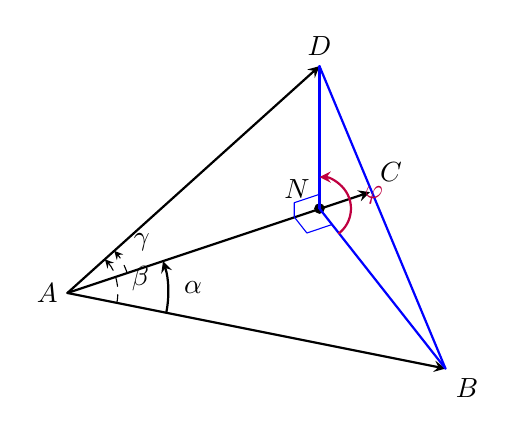
\begin{tikzpicture}[scale=1.6, >=stealth, line join=round, line cap=round]
    \coordinate (A) at (0,0);
    \node[left] at (A) {$A$};
    \coordinate (B) at (3.0,-0.6);
    \coordinate (C) at (2.4,0.8);
    \coordinate (D) at (2.0,1.8);
    
    \draw[thick, ->, black] (A) -- (B) node[below right] {$B$};
    \draw[thick, ->, black] (A) -- (C) node[above right] {$C$};
    \draw[thick, ->, black] (A) -- (D) node[above] {$D$};
    
    \coordinate (N) at (2.0,0.67);
    \fill (N) circle (1.2pt) node[above left] {$N$};
    
    \draw[thick, blue] (N) -- (B);
    \draw[thick, blue] (N) -- (D);
    \draw[thick, blue] (B) -- (D);
    
    % 直角标记
    \draw[blue] ($(N)!0.1!(B)$) -- ($($(N)!0.1!(B)$) + ($(N)!0.1!(A)$) - (N)$) -- ($(N)!0.1!(A)$);
    \draw[blue] ($(N)!0.1!(D)$) -- ($($(N)!0.1!(D)$) + ($(N)!0.1!(A)$) - (N)$) -- ($(N)!0.1!(A)$);
    
    % 标记角
    \draw[->, black, thick] ($(A)+(-11.3:0.8)$) arc (-11.3:18.43:0.8);
    \node[black, right] at ($(A)+(3:0.85)$) {$\alpha$};
    \draw[->, black, dashed] ($(A)+(-11.3:0.4)$) arc (-11.3:42:0.4);
    \node[black, right] at ($(A)+(15:0.45)$) {$\beta$};
    \draw[->, black, dashed] ($(A)+(18.43:0.5)$) arc (18.43:42:0.5);
    \node[black, above right] at ($(A)+(30:0.52)$) {$\gamma$};
    
    \draw[->, purple, thick] ($(N)+(-51.8:0.25)$) arc (-51.8:90:0.25);
    \node[purple, right] at ($(N)+(20:0.3)$) {$\varphi$};
\end{tikzpicture}
\end{center}

\noindent\textbf{【纯几何证明】}\\
在公共棱 $AC$ 上任取点 $N$。在平面 $DAC$ 内作 $ND \perp AC$，交 $AD$ 于点 $D$；在平面 $BAC$ 内作 $NB \perp AC$，交 $AB$ 于点 $B$，连接 $BD$。\\
在 Rt$\triangle AND$（$\angle AND = 90^\circ$）中，$ND = AN \tan\gamma$，$AD = \dfrac{AN}{\cos\gamma}$。\\
在 Rt$\triangle ANB$（$\angle ANB = 90^\circ$）中，$NB = AN \tan\alpha$，$AB = \dfrac{AN}{\cos\alpha}$。\\
二面角的平面角为 $\varphi = \angle DNB$。\\
在斜三角形 $\triangle NDB$ 中，由余弦定理有：
\[ BD^2 = NB^2 + ND^2 - 2 NB \cdot ND \cos\varphi \quad \text{—— 方程 (1)} \]
在三角形 $\triangle ADB$ 中，$\angle DAB = \beta$，由余弦定理有：
\[ BD^2 = AB^2 + AD^2 - 2 AB \cdot AD \cos\beta \quad \text{—— 方程 (2)} \]
联立方程并消去 $BD^2$，整理得：
\[ 2 NB \cdot ND \cos\varphi = (NB^2 - AB^2) + (ND^2 - AD^2) + 2 AB \cdot AD \cos\beta \]
在 Rt$\triangle ANB$ 和 Rt$\triangle AND$ 中，有 $NB^2 - AB^2 = -AN^2$，$ND^2 - AD^2 = -AN^2$。代入得：
\[ NB \cdot ND \cos\varphi = AB \cdot AD \cos\beta - AN^2 \]
两边同除以 $AB \cdot AD$，可得：
\[ \frac{NB}{AB} \cdot \frac{ND}{AD} \cos\varphi = \cos\beta - \frac{AN}{AB} \cdot \frac{AN}{AD} \]
利用三角比定义：$\dfrac{NB}{AB} = \sin\alpha$，$\dfrac{ND}{AD} = \sin\gamma$，$\dfrac{AN}{AB} = \cos\alpha$，$\dfrac{AN}{AD} = \cos\gamma$，代入即得：
\[ \sin\alpha \sin\gamma \cos\varphi = \cos\beta - \cos\alpha \cos\gamma \implies \boxed{\cos\varphi = \frac{\cos\beta - \cos\alpha \cos\gamma}{\sin\alpha \sin\gamma}} \]

\subsection{定理 4：三夹角定理}
\mindsetcard{三夹角模型}{三棱定线面}{射线两两夹角分别为 $\alpha = \angle BAC, \beta = \angle BAD, \gamma = \angle CAD$。设 $AD$ 与平面 $ABC$ 所成线面角为 $\theta$。满足：$\cos\theta = \dfrac{\sqrt{\cos^2\beta + \cos^2\gamma - 2\cos\alpha \cos\beta \cos\gamma}}{\sin\alpha}$。}

\noindent\textbf{【纯几何证明】}\\
设点 $D$ 在平面 $ABC$ 内的正投影为 $H$（即 $DH \perp \text{平面 } ABC$），连接 $AH$，则 $\theta = \angle DAH$。\\
设正投影线 $AH$ 将 $\angle BAC = \alpha$ 分为两部分，$\alpha_1 = \angle BAH$ 和 $\alpha_2 = \angle CAH$，满足 $\alpha_1 + \alpha_2 = \alpha$。\\
对斜线 $AD$、投影线 $AH$ 及底面直线 $AB$ 应用\textbf{三余弦定理}，有：$\cos\beta = \cos\theta \cos\alpha_1 \implies \cos\alpha_1 = \dfrac{\cos\beta}{\cos\theta}$。\\
同理，对斜线 $AD$、投影线 $AH$ 及底面直线 $AC$ 应用\textbf{三余弦定理}，有：$\cos\gamma = \cos\theta \cos\alpha_2 \implies \cos\alpha_2 = \dfrac{\cos\gamma}{\cos\theta}$。\\
由和角公式：$\cos\alpha = \cos(\alpha_1 + \alpha_2) = \cos\alpha_1 \cos\alpha_2 - \sin\alpha_1 \sin\alpha_2 \implies \sin\alpha_1 \sin\alpha_2 = \cos\alpha_1 \cos\alpha_2 - \cos\alpha$。\\
两边平方，并用 $\sin^2 x = 1 - \cos^2 x$ 展开消去 $\cos^2\alpha_1 \cos^2\alpha_2$，整理得：
\[ \cos^2\alpha_1 + \cos^2\alpha_2 - 2\cos\alpha \cos\alpha_1 \cos\alpha_2 = 1 - \cos^2\alpha = \sin^2\alpha \]
将前面 $\cos\alpha_1, \cos\alpha_2$ 的式子代入：
\[ \frac{\cos^2\beta}{\cos^2\theta} + \frac{\cos^2\gamma}{\cos^2\theta} - 2\cos\alpha \frac{\cos\beta \cos\gamma}{\cos^2\theta} = \sin^2\alpha \]
由此解得 $\cos^2\theta = \dfrac{\cos^2\beta + \cos^2\gamma - 2\cos\alpha \cos\beta \cos\gamma}{\sin^2\alpha}$，开方即得：
\[ \boxed{\cos\theta = \frac{\sqrt{\cos^2\beta + \cos^2\gamma - 2\cos\alpha \cos\beta \cos\gamma}}{\sin\alpha}} \]

\newpage

% =====================================================
% 第二章
% =====================================================
\section{立体几何“折叠与折痕”问题不变量模型}

立体几何中的图形折叠问题，其本质是\textbf{绕折痕的旋转运动}。解决此类问题，最关键的动作是：\textbf{寻找“不变量”，并在折叠前后的平面与空间体系间建立长度的桥梁。}

\subsection{折叠模型四大核心守恒量}
\begin{enumerate}
  \item \textbf{折痕（轴）}：折叠运动的旋转轴。折痕上的所有点在折叠前后\textbf{位置完全不动}，所有距离 and 角度保持不变。
  \item \textbf{垂足（中心）}：过动点作折痕的垂线，垂足即为该动点空间旋转轨迹圆的\textbf{圆心}。垂足在折痕上的位置是固定不动的。
  \item \textbf{定长（半径）}：折叠前动点到折痕的距离，等于折叠后该动点到折痕的距离（即旋转轨迹圆的\textbf{半径}）。
  \item \textbf{圆弧轨迹（空间面）}：动点折起后的轨迹是以垂足为圆心、定长为半径、且\textbf{垂直于折痕的平面内}的一个圆弧。
\end{enumerate}

\subsection{典型应用：矩形折叠模型}
\textbf{【经典模型】} 矩形 $ABCD$ 中，$AB=1, BC=\sqrt{3}$。$M$ 是 $AD$ 上的动点。将 $\triangle ABM$ 沿 $BM$ 折起，使 $A$ 到达 $A'$ 且 $A'$ 在底面的正投影 $E$ 落在 $BC$ 上。设 $AM=x$。

\begin{center}
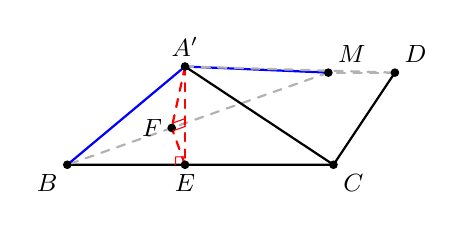
\begin{tikzpicture}[scale=1.3, >=stealth, line join=round, line cap=round]
    \coordinate (B) at (0, 0);
    \coordinate (C) at (2.6, 0);
    \coordinate (D) at (3.2, 0.9);
    \coordinate (M) at (2.55, 0.9);
    \coordinate (E) at (1.15, 0);
    \coordinate (A1) at (1.15, 0.96);
    \coordinate (F) at (1.02, 0.36); 
    
    \draw[thick] (B) -- (C) -- (D);
    \draw[thick, dashed, gray!60] (D) -- (M);
    \draw[thick, dashed, gray!60] (M) -- (B);
    
    \draw[thick, blue] (A1) -- (B);
    \draw[thick, blue] (A1) -- (M);
    \draw[thick] (A1) -- (C);
    \draw[thick, dashed, gray!60] (A1) -- (D);
    
    \draw[thick, dashed, red] (A1) -- (E);
    \draw[thick, dashed, red] (E) -- (F);
    \draw[thick, dashed, red] (A1) -- (F);
    
    \fill (B) circle (1.2pt) node[below left] {\small $B$};
    \fill (C) circle (1.2pt) node[below right] {\small $C$};
    \fill (D) circle (1.2pt) node[above right] {\small $D$};
    \fill (M) circle (1.2pt) node[above right] {\small $M$};
    \fill (E) circle (1.2pt) node[below] {\small $E$};
    \fill (A1) circle (1.2pt) node[above] {\small $A'$};
    \fill (F) circle (1.2pt) node[left] {\small $F$};
    
    \draw[red, thin] ($(E)!0.08!(A1)$) -- ($($(E)!0.08!(A1)$) + ($(E)!0.08!(B)$) - (E)$) -- ($(E)!0.08!(B)$);
    \draw[red, thin] ($(F)!0.08!(A1)$) -- ($($(F)!0.08!(A1)$) + ($(F)!0.08!(M)$) - (F)$) -- ($(F)!0.08!(M)$);
    \draw[red, thin] ($(F)!0.08!(E)$) -- ($($(F)!0.08!(E)$) + ($(F)!0.08!(M)$) - (F)$) -- ($(F)!0.08!(M)$);
\end{tikzpicture}
\end{center}

\noindent\textbf{【核心代数引擎关系】}\\
设 $AM = x$。折起后有守恒量 $A'B = AB = 1$，$A'M = AM = x$。\\
由于 $A'E \perp$ 平面 $BCDM$，且 $BC \subset$ 平面 $BCDM$，所以 $A'E \perp BC$。\\
在 Rt$\triangle A'EB$ 中，有 $A'E^2 = A'B^2 - BE^2 = 1 - BE^2$。\\
在底面，过 $M$ 作 $MM_0 \perp BC$ 于 $M_0$，有 $BM_0 = x, MM_0 = 1$。在 Rt$\triangle EM_0M$ 中，有 $EM^2 = (BE-x)^2 + 1$。\\
在 Rt$\triangle A'EM$ 中，有 $A'M^2 = A'E^2 + EM^2 \implies x^2 = (1-BE^2) + (BE-x)^2 + 1$。\\
化简得：$x^2 = 1 - BE^2 + BE^2 - 2x \cdot BE + x^2 + 1 + 1 \implies 2x \cdot BE = 2 \implies \boxed{BE = \frac{1}{x}}$。\\
由此，我们能极快地求出折起后的高度：$A'E = \sqrt{1 - BE^2} = \boxed{\sqrt{1 - \frac{1}{x^2}}}$。

\subsection{三正弦定理在折叠最值中的“降维”妙用}
在矩形折叠模型中，若要求直线 $CD$ 与折起面 $A'BM$ 所成的线面角 $\alpha$ 的最值，可以进行如下分析：
\begin{enumerate}
  \item \textbf{常规解法}：需要在空间中去作 $CD$ 到平面 $A'BM$ 的投影，找到射影点，建立极其复杂的空间坐标系，计算量极大。
  \item \textbf{同构/三正弦定理直接得出}：
    \begin{itemize}
      \item 视底面 $BCDM$ 为底面 $\beta$，折起面 $A'BM$ 为斜面 $\alpha$（绕交线/折痕 $BM$ 旋转）。
      \item 二面角 $A'-BM-C$ 的平面角为 $\beta$。
      \item 直线 $CD$ 平行于底面内直线 $AB$。在直角三角形 $\triangle ABM$ 中，直线 $AB$ 与折痕 $BM$ 的夹角 $\theta$ 易求：$\sin\theta = \dfrac{AM}{BM} = \dfrac{x}{\sqrt{x^2+1}}$。
      \item 根据\textbf{三正弦定理}，直线 $CD$ 与平面 $A'BM$ 所成的角 $\alpha$ 满足：
        \[ \sin\alpha = \sin\beta \sin\theta \]
      \item 避开了所有寻找空间垂足的步骤，直接将线面角用二面角和底面内夹角表示出来，实现了“降维计算”。
    \end{itemize}
\end{enumerate}

\newpage

% =====================================================
% 第三章
% =====================================================
\section{一元二次方程“根的分布与区间参数”问题}

一元二次方程根的分布及不等式在给定区间上的参数范围问题，是函数部分的核心难点。解题的底层原则是：\textbf{恒成立卡“最坏情况”，有解寻找“最好机会”}。

\subsection{恒成立与有解的最值翻译逻辑}
遇到含有参数的不等式问题，首要动作是确定“谁是自变量，谁是参数”，并将不等式翻译为关于最值的约束条件：

\begin{center}
\renewcommand{\arraystretch}{1.3}
\begin{tabularx}{\linewidth}{p{4.5cm} p{3.2cm} X}
\toprule
\textbf{量词表述} & \textbf{代数翻译} & \textbf{最值约束条件} \\
\midrule
$\forall x \in I,\ f(x) \ge a$ 恒成立 & 所有人都不低于 $a$ & $f(x)$ 在区间 $I$ 上的\textbf{最小值} $f_{\min}(x) \ge a$。 \\
$\forall x \in I,\ f(x) \le a$ 恒成立 & 所有人都不超过 $a$ & $f(x)$ 在区间 $I$ 上的\textbf{最大值} $f_{\max}(x) \le a$。 \\
$\exists x \in I,\ f(x) \ge a$ 有解 & 只要有一个人不低于 $a$ & $f(x)$ 在区间 $I$ 上的\textbf{最大值} $f_{\max}(x) \ge a$。 \\
$\exists x \in I,\ f(x) \le a$ 有解 & 只要有一个人不超过 $a$ & $f(x)$ 在区间 $I$ 上的\textbf{最小值} $f_{\min}(x) \le a$。 \\
\bottomrule
\end{tabularx}
\end{center}

\subsection{一元二次方程根在区间 $[k_1, k_2]$ 上的“五因子”扫描树}
对于二次函数 $f(x) = ax^2 + bx + c\ (a > 0)$，若其两个实根都在区间 $[k_1, k_2]$ 内，切忌盲目乱写条件。我们必须按\textbf{“五因子扫描树”}逐项排查：

\begin{enumerate}
  \item \textbf{开口方向}：确认 $a > 0$（若 $a$ 含参需讨论退化为一次方程的情况）。
  \item \textbf{判别式}：确保有实根，$\Delta = b^2 - 4ac \ge 0$。
  \item \textbf{对称轴}：对称轴必须落在给定区间内，即 $k_1 \le -\dfrac{b}{2a} \le k_2$。
  \item \textbf{端点值}：区间左端点和右端点的函数值必须非负，即 $f(k_1) \ge 0$ 且 $f(k_2) \ge 0$。
  \item \textbf{参数讨论}：讨论参数变动引起的轴滑动（“轴动区间定”或“轴定区间动”）。
\end{enumerate}

\[
\text{两个根在 } [k_1, k_2] \text{ 内} \iff 
\begin{cases}
  \Delta \ge 0 \\
  k_1 \le -\dfrac{b}{2a} \le k_2 \\
  f(k_1) \ge 0 \\
  f(k_2) \ge 0
\end{cases}
\]

\subsection{三大通用破解法：分离参数与主参换位}
\begin{itemize}
  \item \textbf{方法 1：分离参数法} \\
    若不等式中参数 $a$ 能够干净地分离出来，形如 $a \le g(x)$ 恒成立，则直接转化为求 $g(x)$ 的最小值，即 $a \le g_{\min}(x)$。此法为通法，能避开繁琐的分类讨论。
  \item \textbf{方法 2：分类讨论法（轴动区间定）} \\
    当无法分离参数时，必须以\textbf{对称轴与区间的相对位置}为基准进行讨论。通常分为三段：轴在区间左侧、轴在区间内部、轴在区间右侧。结合开口方向，求出每段的最小值，最后取交集或并集。
  \item \textbf{方法 3：主参换位法（主元法）} \\
    当自变量 $x$ 的次数较高（如二次），但参数 $a$ 的次数仅为一次时，我们应果断\textbf{颠倒主仆关系}，将原式看作关于参数 $a$ 的一次函数。\\
    若 $f(x, a) \ge 0$ 对 $\forall a \in [a_1, a_2]$ 恒成立，则将其整理为 $g(a) = A(x)a + B(x) \ge 0$。由于一次函数在闭区间上的最值只能在端点处取得，故只需满足两个端点处非负：
    \[ g(a_1) \ge 0 \quad \text{且} \quad g(a_2) \ge 0 \]
    这可以将复杂的二次讨论瞬间降维为两个简单的一次不等式组！
\end{itemize}

\newpage

% =====================================================
% 第四章
% =====================================================
\section{函数同构与“指对同构”技术}

同构变形是攻克导数压轴题和高一函数提升题的终极“神技”。其本质是\textbf{利用对应函数结构的一致性，借助单调性将复杂的代数关系还原为自变量的简单大小关系}。

\subsection{同构变形的核心流程}
若能通过代数变形将关于 $x_1, x_2$ 的等式或不等式整理为两边代数表达结构完全一致的形式：
\[ F(x_1) \ge F(x_2) \]
那么，这个相同的代数结构 $F(t)$ 就是我们要构造的辅助函数。
\begin{itemize}
  \item 若 $F(t)$ 在相应区间上单调递增，则 $F(x_1) \ge F(x_2) \iff x_1 \ge x_2$。
  \item 若 $F(t)$ 在相应区间上单调递减，则 $F(x_1) \ge F(x_2) \iff x_1 \le x_2$。
\end{itemize}

\subsection{指对同构的“双通道恒等式”}
指对同构的核心难点在于：式子中既含有指数式（以 $e^x$ 为代表），又含有对数式（以 $\ln x$ 为代表）。我们必须通过\textbf{“双通道恒等式”}强行将两边化为同一底数：

\begin{center}
\renewcommand{\arraystretch}{1.5}
\begin{tabularx}{0.8\linewidth}{c X}
\toprule
\textbf{变换通道} & \textbf{恒等式关系} \\
\midrule
\textbf{指数通道} & $x = e^{\ln x}$ （将代数项 $x$ 强行化为以 $e$ 为底的指数式） \\
\textbf{对数通道} & $x = \ln(e^x)$ （将代数项 $x$ 强行化为对数式） \\
\bottomrule
\end{tabularx}
\end{center}

\subsection{三大经典同构函数族}
在实际解题中，我们主要寻找以下三种经典同构结构：

\begin{enumerate}
  \item \textbf{$t e^t$ 型（积型）} \\
    例如：若方程为 $x e^x = y \ln y$。\\
    我们利用指数通道，将右边的 $y \ln y$ 化为：$\ln y \cdot e^{\ln y}$。\\
    此时原方程化为：$x e^x = \ln y \cdot e^{\ln y}$。\\
    构造辅助函数 $F(t) = t e^t$，则有 $F(x) = F(\ln y)$。由于当 $t > 0$ 时 $F(t)$ 单调递增，故直接有 $\boxed{x = \ln y}$。
    
  \item \textbf{$t + \ln t$ 型（和型）} \\
    例如：若方程为 $x e^x = y$。两边同时取自然对数，得：$\ln x + x = \ln y$。\\
    利用对数通道，将 $x$ 替换为 $\ln(e^x)$，则有：$\ln x + \ln(e^x) = \ln y$（结构尚不完美）。\\
    若原式为 $x + \ln x = e^u + u$，直接构造 $F(t) = t + \ln t$。\\
    对于 $x e^x \ge y$，取对数得 $x + \ln x \ge \ln y \implies \ln(e^x) + e^x \ge \ln y + y$。我们发现两边都符合 $t + e^t$ 的形式，构造 $F(t) = t + e^t$，则有 $F(x) \ge F(\ln y) \implies \boxed{x \ge \ln y}$。
    
  \item \textbf{$\dfrac{\ln t}{t}$ 型（商型）} \\
    若等式两侧呈现“分子为对数，分母为代数项”的特征，如 $\dfrac{\ln x_1}{x_1} = \dfrac{\ln x_2}{x_2}$。\\
    直接构造辅助函数 $F(t) = \dfrac{\ln t}{t}$。在区间 $(0, e)$ 上单调递增，在 $(e, +\infty)$ 上单调递减。
\end{enumerate}

\newpage

% =====================================================
% 第五章
% =====================================================
\section{对数函数与结构转化（高一免导数法）}

在高一阶段，我们还没有学习导数，但经常会遇到对数函数的多变量零点问题（如极值点偏移的简化版）。此时，我们必须利用\textbf{“对称换元”}和\textbf{“结构变形”}进行免导数分析。

\subsection{多变量对数零点问题的对称换元法}
若函数 $f(x) = \ln x - kx$ 存在两个零点 $x_1, x_2\ (x_1 < x_2)$。要求求出 $x_1 x_2$ 或 $x_1+x_2$ 的取值范围，可以按以下步骤进行：
\begin{enumerate}
  \item \textbf{第一步：列出零点等式}
    \[ \ln x_1 = k x_1,\quad \ln x_2 = k x_2 \]
  \item \textbf{第二步：消去参数 $k$}
    两式相除或相减：
    \[ k = \frac{\ln x_1}{x_1} = \frac{\ln x_2}{x_2} \implies \frac{\ln x_1}{\ln x_2} = \frac{x_1}{x_2} \quad \text{或} \quad \ln x_2 - \ln x_1 = k(x_2 - x_1) \implies k = \frac{\ln\dfrac{x_2}{x_1}}{x_2 - x_1} \]
  \item \textbf{第三步：对称换元}
    设比值 $t = \dfrac{x_2}{x_1} > 1$。我们将 $x_1, x_2$ 用 $t$ 和 $k$ 进行表示：
    由于 $\ln t = k(x_2 - x_1) = k x_1(t - 1) \implies x_1 = \dfrac{\ln t}{k(t - 1)}$，同理 $x_2 = \dfrac{t \ln t}{k(t - 1)}$。\\
    那么乘积为：$x_1 x_2 = \dfrac{t \ln^2 t}{k^2(t-1)^2}$。由于 $k = \dfrac{\ln x_1}{x_1}$，我们可以利用无参结构进行化简，或证明单调性，绕开导数直接得出比值 $t$ 的范围，从而锁定乘积或和的界限。
\end{enumerate}

\subsection{底数转化与图像直观}
对于不同底数的对数式，第一步必须化同底。
\begin{itemize}
  \item \textbf{换底公式}：$\log_a b = \dfrac{\ln b}{\ln a}$。
  \item \textbf{图像叠加}：方程 $\log_a x = \log_b(x-1)$ 的解的个数问题，应通过画出两个对数函数的图像，观察它们的交点变化。
\end{itemize}

\newpage

% =====================================================
% 第六章
% =====================================================
\section{解三角形边角压轴与几何不等式}

在解三角形的压轴大题中，核心难点在于\textbf{边角关系的灵活转化}以及结合不等式求取最值。

\subsection{边角互化决策导航}
拿到一道题，首先要决策是“全化为边”还是“全化为角”：

\begin{center}
\renewcommand{\arraystretch}{1.3}
\begin{tabularx}{\linewidth}{p{4.0cm} p{4.0cm} X}
\toprule
\textbf{特征类型} & \textbf{首选决策} & \textbf{核心公式依据} \\
\midrule
含有三边的一次或二次混合式，没有角度的和差 & \textbf{角化边}（全化为边） & 余弦定理：$\cos C = \dfrac{a^2+b^2-c^2}{2ab}$；正弦定理边角代换。 \\
含有角度的和差，或有 $\sin A, \cos B$ 等乘积项 & \textbf{边化角}（全化为角） & 正弦定理：$a = 2R\sin A$；结合内角和 $A+B+C=\pi$ 消角。 \\
\bottomrule
\end{tabularx}
\end{center}

\subsection{解三角形最值与不等式三大利器}
在求周长、面积或边长最值时，我们主要借助以下三个不等式工具：

\begin{enumerate}
  \item \textbf{均值不等式（AM-GM）} \\
    在已知角 $C$ 及对边 $c$ 时，由余弦定理有：$c^2 = a^2 + b^2 - 2ab \cos C$。\\
    由于 $a^2 + b^2 \ge 2ab$，代入可得：
    \[ c^2 \ge 2ab - 2ab \cos C = 2ab(1 - \cos C) \implies ab \le \frac{c^2}{2(1 - \cos C)} \]
    当且仅当 $a = b$（等腰三角形）时取得等号。由此可求出面积 $S = \dfrac{1}{2} ab \sin C$ 的最大值。
    
  \item \textbf{柯西不等式（Cauchy-Schwarz）} \\
    用于求周长 $a+b+c$ 的范围。\\
    若已知 $a^2 + b^2 = m$，则由柯西不等式：
    \[ (a + b)^2 \le (1^2 + 1^2)(a^2 + b^2) = 2(a^2 + b^2) = 2m \implies a+b \le \sqrt{2m} \]
    此法对于求双变量线性组合的最值极其迅速。
    
  \item \textbf{辅助角公式与三角函数有界性} \\
    若将所有的边都通过正弦定理化为关于角 $A$ 的三角函数：
    \[ a+b = 2R\sin A + 2R\sin B = 2R\left[\sin A + \sin(C-A)\right] \]
    利用和差化积或辅助角公式整理为 $A \sin(A + \theta)$ 的单角形式，利用 $A \in (0, \pi)$ 的范围直接求出三角函数的值域。
\end{enumerate}

\newpage
\label{LastPage}
\end{document}
